\documentclass[journal,12pt,twocolumn]{IEEEtran}
\usepackage{amsmath,amsfonts,amssymb,float}
\usepackage{graphicx}
\bibliographystyle{IEEEtran}
\vspace{3cm}
\title{NCERT Discrete}
\author{Pragnidhved Reddy\\EE23BTECH11050}
\date{}
\parindent 0px
\begin{document}
\maketitle
\newpage
\bigskip
\textbf{Question 10.5.2.8:}\\
An AP consists of $50$ terms of which $3^{rd}$ term is $12$ and the last term is $106$. Find the $29^{th}$ term.\\
\textbf{Solution :}\\
\begin{table}[H]
\centering
\begin{tabular}{|c|c|c|}\hline
\textbf{Parameter} & \textbf{Value} & \textbf{description}\\ \hline
$x(3)$ & $12$ & Third term\\ \hline
$x(50)$ & $106$ & Last term\\ \hline
$x(0)$ & $?$ & Zeroth term \\ \hline
$d$ & $?$ & Common difference\\ \hline
$x(n)$ & $[x(0)+nd]u(n)$ & general term \\ \hline
\end{tabular}
\caption{Input parameters}
\end{table}
\begin{align}
x(3)=x(0)+3d\\
x(50)=x(0)+50d
\end{align}
By solving (1) and (2), we get
\begin{align}
\implies &d=2\\
\implies &x(0)=6
\end{align}
From the table
\begin{align}
x(n)&=[x(0)+nd]u(t)\\
\implies x(n)&=(6+2n)u(t)\\
\end{align}
Finding x(29)
\begin{align}
x(29)&=x(0)+29(2)\\
\implies x(29)&=64
\end{align}
Finding the Z-transform
\begin{align}
X(z)&=\sum_{k=-\infty}^{\infty}x(n)\times u(t)\times z^{-n}\\
\implies X(z)&=\sum_{k=0}^{\infty}x(n)\times z^{-n}\\
\implies X(z)&=\frac{6-8z^{-1}}{(1-z^{-1})^2} \quad \abs{|z|}>1
\end{align}
\begin{figure}[h!]
    \centering
    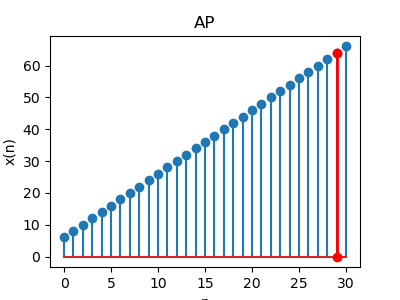
\includegraphics{figs/plot.png}
    \caption{graph of the given AP}
    \label{fig:1}
\end{figure}
\end{document}
